
\section{How low can we go?}\label{sec:low_O2}

Ruthenium dioxide can oxidize water at remarkably low overpotential in acidic electrolyte\cite{Miles1976, Reier2017}. However, it is not particularly stable, with anywhere from 0.01\% to 10\% of the current going to \ch{Ru} dissolution, depending on the preparation and experimental conditions\cite{Roy2018}. It is also used as a super-capacitor material\cite{Gonzalez2016} due to a very high pseudo-capacitance. This pseudocapacitance is due to the many redox transitions on the surface sites of \ch{RuO2} as well as the tendency of \ch{RuO2}, especially amorphous \ch{RuO2}, to form nano-scale interconnected domains, the surface of all of which are electrolytically accessible\cite{Yoshida2013}. In the previous Section, I illustrated that it is necessary to measure the \ch{O2} when studying OER catalysts. Together, the instability and high pseudo-capacitance (and thus large transient charging current) make this especially true for \ch{RuO2}-based electrodes. With this in mind, as well as the ability to do very sensitive isotope-labeling experiments, described in the next Section, we started a collaboration with Reshma Rao and professor Yang Shao-Horn at MIT to use our EC-MS system to study OER on \ch{RuO2}. One of the main goals was to see how low the onset potential for OER actually is.

\subsection{Sputtered \ch{RuO2} films}

\begin{figure}[b!]
	\centering
	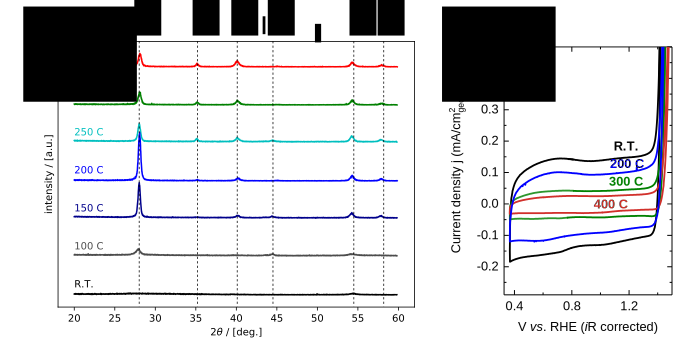
\includegraphics[width=0.8\textwidth]{04_Oxygen/fig/RuO2_film_char.png}
	\caption{Characterization of \ch{RuO2} films sputter-deposited at various temperatures. \textbf{(a)}, Grazing-incidence x-ray diffraction spectra. The theoretical peak positions of rutile \ch{RuO2} are indicated. \textbf{(b)} Cyclic voltammatry at a scan rate of 10 mV/s.}
	\label{fig:RuO2_char}
\end{figure}

To check whether and how activity, stability, and lattice oxygen involvement varied with crystallinity, we sputtered \ch{RuO2} at various temperatures. Reshma and I made the first samples together when she visited DTU in September 2018. We sputtered \ch{RuO2} by reactive sputtering of a Ru sputter target with a magnetron sputter power of 300 W at a total pressure of 3 mTorr consisting of 80\% Ar and 20\% \ch{O2}. We sputtered \ch{RuO2} films of 25 nm nominal thickness (calibrated by quartz crystal microbalance) on a 5 nm Ti sticking layer on glassy carbon disks. The films are characterized by grazing-incidence x-ray diffraction (GIXRD) and cyclic voltammatry in Figure \ref{fig:RuO2_char}.

\ch{RuO2} sputtered at room temperature (RT) appears amorphous, with no peaks visible in the diffractogram (Figure \ref{fig:RuO2_char}a). The films become more crystalline at higher sputtering temperature. However, while all the other peaks increase in intensity from RT to 400$^\circ$C sputtering, the (110) peak passes through a maximum at a sputtering temperature of 200$^\circ$C. This might indicate that a preferential orientation occurs at the right sputtering temperatures.

The relative surface areas of the samples, measured by electrochemical capacitance, however, decreases monotonically with higher sputtering temperature (Figure \ref{fig:RuO2_char}b). All of the films appear to be quite rough. Using a specific pseudo-capacitance (double-layer capacitance + redox charging) of 200 $\mu$F/cm$^2$ (this assumption is discussed in Subsection \ref{subsec:TOF})\cite{Yoshida2013}, the roughnesses factors go from $\approx$9 for the 400$^\circ$C-sputtered film to $\approx$60 for the RT-sputtered film. %Interesting, this roughness is on a 1-nm scale or smaller, as all films appear flat in AFM.

\begin{figure}[t]
	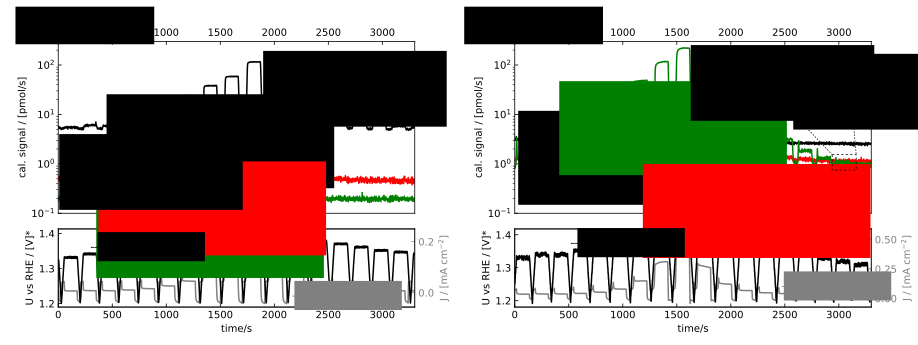
\includegraphics[width=1\textwidth]{04_Oxygen/fig/Reshma1_activities.png}
	\caption{Activity measurement of a \ch{RuO2} film sputtered at room temperature in 0.1 M \ch{HClO4} in \textbf{(a)} natural (99.8\% \ch{H2^{16}O}) water, and \textbf{(b)} 97\% \ch{H2^{18}O} labeled water.}
	\label{fig:Reshma1_activities}
\end{figure}


To measure the OER activities of the sputtered films in 0.1 M \ch{HClO4}, we scanned the potential at 5 mV/s from a ``resting potential'' of 1.2 V vs RHE to a working potential at which the OER measurement is made, holding each potential for 2 minutes. This was done to let the \ch{O2} signal reach a steady state at each potential and fall to the background level between activity measurements. The RHE potential of the reference electrode was always measured in the same electrolyte and the same setup using a platinum electrode and saturating the electrolyte in \ch{H2}, as described in Section \ref{subsec:examples}. The \ch{O2} signal was calibrated by 5-minute constant-current OER steps (20 $\mu$A, 50 $\mu$A, and 100 $\mu$A) from a rutile \ch{IrO2} electrode measured in the setup on the same day, since \ch{IrO2} is known to be much more stable than \ch{RuO2}\cite{Reier2017}.

The activity measurement for an R.T.-sputtered film is shown in Figure \ref{fig:Reshma1_activities}a. \ch{O2} production is stable during each 2-minute potential hold, giving a nice ''square-wave'' shape to the m/z=32 signal. The \ch{O2} production rate follows a neat Tafel relationship with applied potential, i.e. for a constant linear increase in potential step, the \ch{O2} signal increases by a constant factor. Specifically, the \ch{O2} production rate increases by a factor $\approx$ 2 for each 10 mV step in potential. More commonly, this is stated in the reciprocal form, as the extra potential required for a factor 10 increase in activity (a ``decade''), referred to as the Tafel slope. Here, the Tafel slope is $\approx$ 30 mV per decade

An oxygen signal is detectable down to 1.33 V vs RHE, a nominal overpotential of 100 mV. This was, to the best of our knowledge, already a record for detection of \ch{O2} from water oxidation. 

It should be emphasized that, while \ch{RuO2} is highly active, and the room-temperature-deposited film has the highest activity of the sputtered films, in line with its high roughness factor, we have no reason to believe that our \ch{RuO2} is more active than \ch{RuO2} reported in the literature. The detection of \ch{O2} at very low overpotential should, instead, be viewed as an accomplishment of the technique - specifically, the exceptionally high sensitivity of the chip-based EC-MS setup to gaseous products.

The detection limit of \ch{O2} is limited by the background of the m/z=32 signal, which is probably set by outgassing of the MS filament or other components in the vacuum chamber, or extremely small leaks. Since the background is thus dominated by natural \ch{O2}, which is 99.5\% \ch{^{16}O2}, the background at m/z=34 (\ch{^{16}O^{18}O}) and m/z=36 (\ch{O^{18}O2}) are considerably lower - by more than an order of magnitude comparing m/z=36 and m/z=32 as seen in \ref{fig:Reshma1_activities}a. Thus, additional sensitivity can be gained by isotopically labeling the oxygen in the electrolyte, and thus labeling the electrochemically produced \ch{O2}.

Figure \ref{fig:Reshma1_activities}b shows an activity measurement of the same sample in 0.1 M \ch{HClO4} in 97\% \ch{H2^{18}O}. The y-axis in the top panel is on the same log-scale as that in Figure \ref{fig:Reshma1_activities}a so that the activities and backgrounds are directly comparable. Unfortunately, the m/z=36 background increases with the change of electrolyte, indicating that the \ch{O2} background in general comes partly from reaction of \ch{H2O} molecules, originating from the electrolyte, on the filament of the mass spectrometer. Due to this increase in background, the \ch{O2} detection limit is only improved by less than an order of magnitude. This, however, enables clear detection of \ch{O2} at 1.32 V vs RHE, a nominal overpotential of 90 mV.

It should be mentioned that the isotopic composition of the \ch{O2} produced in these experiments in labeled electrolyte always reflected the isotopic composition of the electrolyte within uncertainty thereof. In other words, there was no obvious ``isotope'' signal consisting of a transient excess of \ch{^{16}O} coming form the \ch{Ru^{16}O2} electrode. Such isotope signals are, however, observed in more sensitive experiments, and are the subject of the next two Sections.

\begin{figure}[t]
	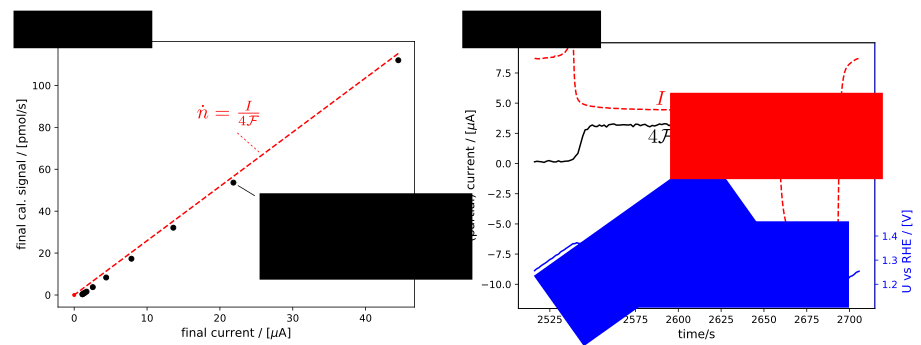
\includegraphics[width=1\textwidth]{04_Oxygen/fig/flux_and_current.png}
	\caption{Closer look at the activity measurement of a \ch{RuO2} film sputtered at room temperature in 0.1 M \ch{HClO4} in  natural (99.8\% \ch{H2^{16}O}) water. \textbf{(a)} Comparison of the averaged current and the \ch{O2} flux as measured during the final 30 seconds of each constant-potential step. The dotted line  \textbf{(b)} comparison of the instantaneous current (red) and \ch{O2} partial current density (black) during the activity measurement at 1.37 V vs RHE.}
	\label{fig:flux_and_current}
\end{figure}

As mentioned above, a concern with OER measurements in general, and in particular on \ch{RuO2}-based materials due to the high charging current and instability, is weather all of the electrode current is going to oxygen evolution. Figure \ref{fig:flux_and_current}a shows the value of the calibrated \ch{O2} signal vs the measured electrode current, averaged over the last 30 seconds of each 2-minute potential hold in Figure \ref{fig:Reshma1_activities}a. The theoretical line assuming 100\% Faradaic efficiency for \ch{O2} production is shown in red. The experimental data has the same slope as the theoretical line, but with a slight offset, with slightly less \ch{O2} than expected from the current. This is inconsistent with a significant dissolution current, as \ch{RuO2} dissolution increases with the current\cite{Cherevko2016}.

A more likely source of this offset is the charging current. Figure \ref{fig:flux_and_current}b shows a zoom-in of the potential step at 1.37 V vs RHE from Figure \ref{fig:Reshma1_activities}a. The calibrated \ch{O2} signal is multiplied by 4$\mathcal{F}$ to give a partial current density, and is plotted on the same axis (left y-axis) as the measured current. Here, we see that the measured current is dominated by capacitance while the potential is being scanned. This capacitive charging current continues during the potential hold, with the current only slowly approaching a steady state. The shape of the current during the constant-potential period is not completely exponential, but has a long tail, indicating that some parts of the electrode are harder to charge than others. In contrast, the \ch{O2} signal is stable during the potential hold. This comparison indicates that some of the current can still be contributed to the charging of the electrode even at the end of the two-minute potential hold.

\subsection{Hydrogen-bubble-template \ch{Ru} foam}\label{subsec:Ru_foam}

\begin{figure}[t!]
	\centering
	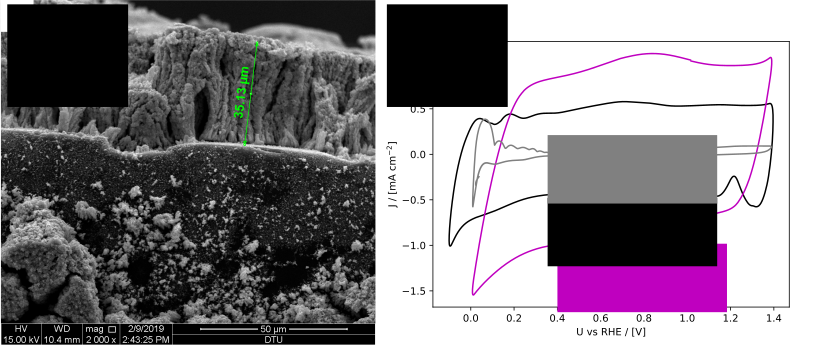
\includegraphics[width=0.9\textwidth]{04_Oxygen/fig/Ru_foam_characterization.png}
	\caption{\textbf{(a)} SEM image of Ru foam. \textbf{(b)} Cyclic voltammatry in 0.1 M \ch{HClO4} of a polycrystalline Pt electrode (gray), a room-temperature sputtered \ch{RuO2} film (black), and Ru foam (magenta). Note the different scan rates. The features just after the cathodic and anodic turns on the R.T. \ch{RuO2} cyclic voltammagram are artifacts of the electrode arrangement in the EC-MS setup.}
	\label{fig:Ru_foam_char}
\end{figure}

To see if we could push the limit of \ch{O2} detection to even lower overpotentials, we synthesized a high-surface-area ruthenium foam by the hydrogen-bubble template method. Choongman Moon and I made the first ones after useful input from Anna Winiwarter, who had optimized a procedure for depositing palladium foam (used for Paper \ref{Winiwarter2019}). Choongman made all of the subsequent films Briefly, a glassy carbon disk suspended by a copper wire fastened with a u-cup and Teflon table was immersed in a solution of 10 mM \ch{RuCl3} and 0.1 M \ch{HClO4}, opposite and parallel to a \ch{RuO2}/p+Si counter electrode held in place by gold wire. A bias of -6 V was applied to the working electrode with respect to the counter electrode for 10 minutes. Metallic Ru is deposited by reduction of the \ch{RuCl3} in solution. This results in an Ru ``foam'' layer that is extremely porous, as the Ru deposition is mass-transport limited and occurs simultaneously with rapid bubble formation by hydrogen evolution. Figure \ref{fig:Ru_foam_char}a shows a cross-sectional SEM image of the Ru foam.

\begin{figure}[b!]
	\centering
	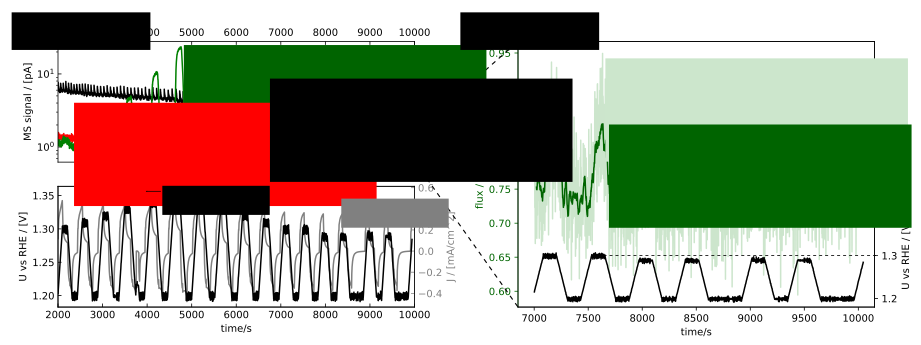
\includegraphics[width=1\textwidth]{04_Oxygen/fig/Ru_foam_activity.png}
	\caption{\textbf{(a)} EC-MS plot with raw MS data from an activity measurement at low overpotentials on the \ch{Ru} foam in 0.1 M \ch{HClO4} in 97\% \ch{H2^{18}O}. \textbf{(b)} Zoom-in on the lowest overpotentials, with the calibrated \ch{^{18}O2} (m/z=36) signal (faint green). The solid green trace is a 15-point moving-average smoothing of the \ch{^{18}O2} signal.}
	\label{fig:Ru_foam_activity}
\end{figure}

Figure \ref{fig:Ru_foam_char}b shows cyclic voltammatry of the \ch{Ru} foam, with a \ch{RuO2} film sputtered at room temperature and a polycrystalline platinum stub included for comparison. Notice the different scan rates, necessary because the charging current of the Ru foam at 50 mV/s would max out the available bias between the working and counter electrodes in the EC-MS setup. The electrochemically accessible surface area is clearly much higher than that of the room-temperature sputtered \ch{RuO2}, which already has a high roughness factor. Assuming the same specific capacitance of 200 $\mu$F/cm$^{2}$\cite{Yoshida2013}, the roughness factor of the Ru foam is on the order of 2000.

The results of an activity test on a Ru foam sample in labeled electrolyte are shown in Figure \ref{fig:Ru_foam_activity}a. \ch{^{18}O2} is detectable down to very low overpotentials. Note in the bottom panel that the charging current overwhelms the OER current, making the measurement of \ch{O2} absolutely necessary to determine the activity at low overpotentials. At the lowest potential measured, 1.29 V vs RHE, the signal can barely be discerned from the noise in the m/z=36 signal. This data point was repeated a total of four times with varying resting times in between in order to increase confidence that there is indeed a signal. The signal is more apparent when the data is smoothed with a 15-point moving average, which is shown as the solid green trace in Figure \ref{fig:Ru_foam_activity}b. Thus, we can claim to have detected \ch{O2} produced electrochemically at 1.29 V vs RHE, just 60 mV above the standard equilibrium potential.


\subsection{Turn-over-frequencies}\label{subsec:TOF}

\begin{figure}[b!]
	\centering
	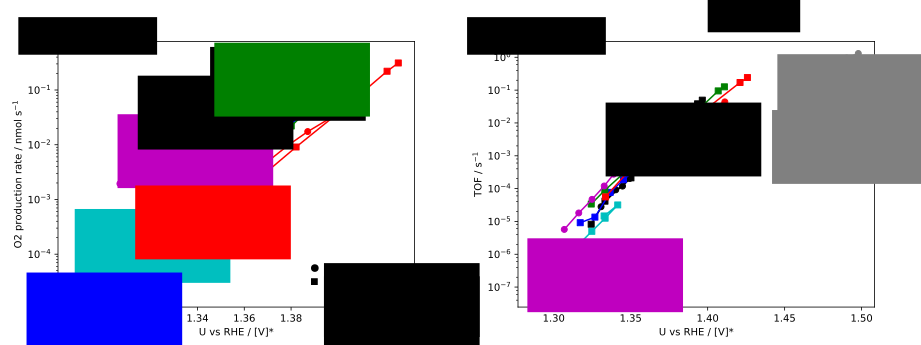
\includegraphics[width=1\textwidth]{04_Oxygen/fig/Ru_TOF.png}
	\caption{\textbf{(a)} \ch{O2} production rate as a function of potential for all measured sputtered \ch{RuO2} films and electrodeposited \ch{Ru} foams. \textbf{(b)} TOF for films and foams, assuming a specific capacitance of 200 $\mu$A/cm$^2$ and a an active site density of 2 per nm$^2$, correspondint to CUS sites on \ch{RuO2}(110)\cite{Rao2017a}. [A] TOF for 3 nm \ch{RuO2} nanoparticles are from Paoli et al, Reference \citen{Paoli2015}.}
	\label{fig:Ru_TOF}
\end{figure}

Figure \ref{fig:Ru_TOF}a shows the \ch{O2} production rate, measured at m/z=32 or m/z=36 signal depending on the labeling of the electrolyte, averaged over the last 30 seconds of 2-minute potential holds for a number of \ch{RuO2} sputtered films and \ch{Ru} foams. All of the geometric areas were 0.196 cm$^2$. There is a large variation spanning approximately three orders of magnitude, with the \ch{Ru} foams producing \ch{O2} at a much higher rate at a given potential. This can, however, be almost fully explained by surface area. In Figure \ref{fig:Ru_TOF}, the \ch{O2} production rate is normalized to the estimated number of active sites. This estimate was made using the following assumptions:

\begin{itemize}
	
	\item Assume a density of active sites equal to the density of CUS sites on the \ch{RuO2}(111) surface.
	
	\item Assume all surface contributing to the capacitance is active.
		
	\item Use the value 200 $µ$F/cm$^2$ determined by SAXS by Yoshida et al, Reference \citen{Yoshida2013}, applied to the portion of the CV's between 1.2 and 1.3 V vs RHE.
\end{itemize}

The first assumption seems reasonable, as (110) is the most stable surface of \ch{RuO2}, the CUS site is believed to be the active site\cite{Reier2017, Rao2017a}, and metallic Ru will have an oxidized surface at the potentials of interest. However, direct determination of the actual active sites would be highly useful. The STM method described Bandarenka and co-workers is a promising strategy\cite{Pfisterer2017}.

The second assumption implies that there are no mass transport limitations in (\ch{H2O}) and out (\ch{H+} and \ch{O2}) of the porous structures of the amorphous \ch{RuO2}. This assumption is reasonable at the low current densities accessible in the EC-MS setup, but might break down at higher current densities. 

The third assumption is based on a study using small-angle x-ray scattering (SAXS) to estimate the combined surface area of the condensed \ch{RuO2} aggregates in a series of hydrous \ch{RuO2} electrodes\cite{Yoshida2013}. The authors of that study found that comparing the electrochemical charging current to the aggregate surface area thus estimated yielded a constant specific capacitance of 200 $\mu$F/cm$^2$, of which they estimate that $\approx$ 80 $\mu$F/cm$^2$ is double-layer capacitance and $\approx$ 120 $\mu$F/cm$^2$ is due to surface redox transitions. Here, I have implicitly assumed that all \ch{Ru} and \ch{RuO2} surfaces have the same double-layer and redox specific charging densities in the potential range 1.2 to 1.3 V vs RHE, chosen because all measurement datasets include potential scans spanning this range.

Figure \ref{fig:Ru_TOF}b shows the turn-over-frequencies thus calculated. All of the \ch{RuO2} and \ch{Ru} samples converge on a common curve with $\approx$ 1 order of magnitude scatter. This adds validity to the assumptions made above, and suggest that the active sites are the same on the different materials. The curve has a slowly changing slope, with a Tafel slope of approximately 30 mV/decade at the upper end (1.38-1.42 V vs RHE), and a Tafel slope of approximately 20 mV/decade at the low overpotential range (1.30-1.34 V vs RHE). 

It is informative to compare these TOF values to TOF values measured and calculated by other means. In Reference \citen{Paoli2015}, Paoli et al report TOF values for mass-selected 3 nm \ch{RuO2} nanoparticles deposited with the same cluster source method used in Paper \ref{Roy2018} and described briefly in Subsection \ref{subsec:NiFe}. Just like in that study, Paoli et al determine the number of active sites via the loading of the nanoparticles, which is known via the deposition current and the size of the nanoparicles. They compare two assumptions for the number of active sites: (1) that all Ru atoms are active sites (TOF$_{\text{bulk}}$), and (2) that only the Ru atoms at the surface of the \ch{RuO2} nanoparticles are active sites  (TOF$_{\text{surf}}$). These two TOF values are co-plotted with the present results in Figure \ref{fig:Ru_TOF}a. The TOF$_{\text{surf}}$ results for the nanoparticles broadly continue the trend observed for the electrodeposited foams and sputtered films, with a further increase in Tafel slope at higher potentials, to about 60 mV/decade at 1.46 - 1.50 V vs RHE. This further supports the assertion that the active sites are similar however Ru or \ch{RuO2} are prepared, and that activity is limited to the surface, though this surface area can be very large.

Note that the problem of uneven potential distribution described in Subsection \ref{subsec:disadvantages} puts some uncertainty on the activity measurements at higher current densities. Due to resistance across the electrolyte film between the electrode and the chip, the potential on the side of the working electrode closest to the counter electrode can be somewhat higher than the measured potential. Taking this into account, the activity at high current densities is likely overestimated, meaning that the curves should bend more towards higher Tafel slopes at higher current densities. If this is the case, it would actually improve the agreement with the nanoparticles. Fortunately, it is the measured behavior at low current densities, which is more reliable, which is of the most interest in this context.

The changing Tafel slope has mechanistic implications\cite{Shinagawa2015}. Briefly, the oxygen evolution reaction consists of four steps, most simply written as\cite{Man2011, Busch2016}:

\begin{align}
\ch{H2O + $*$ -> $*$ OH + (H+ + e-)}\label{rxn:OER_s1}\\
\ch{$*$ OH -> $*$ O + (H+ + e-)}\label{rxn:OER_s2}\\
\ch{$*$ O + H2O -> $*$ OOH + (H+ + e-)}\label{rxn:OER_s3}\\
\ch{$*$ OOH -> $*$ + O2 + (H+ + e-)}\label{rxn:OER_s4}
\end{align}

In the limit that one of these steps, step $i$, is slower than the rest, then the rate is

\begin{equation}
r = k^0_i\theta_{i-1}\exp\left(\frac{\mathcal{F}}{RT}\alpha_i(U-U^\circ_i)\right)\,,\label{eq:rate}
\end{equation}
where $k^0_i$ is the rate constant for the $i$'th step, $U^\circ_i$ is its equilibrium potential. $\theta_{i-1}$ is the coverage of the reactant to that step, i.e., $\theta_0 = \theta_{*}$, $\theta_1 = \theta_{* \ch{OH}}$, $\theta_2 = \theta_{* \ch{O}}$, and $\theta_3 = \theta_{* \ch{OOH}}$. Finally, $\alpha_i$ is the symmetry factor to the reaction. The symmetry factor is the ratio of the change of the activation barrier of an elementary electrochemical reaction to the change in its overall $\Delta G$ resulting from a change in potential\cite{Bard2001}. Equation \ref{eq:rate} is thus an Arrhenius equation, with the activation barrier
\begin{equation}
E_{a,i} = - \alpha_i\mathcal{F}(U - U^\circ_i)\,.
\end{equation}
Symmetry factors for elementary electrochemical steps are typically on the order of 0.5, meaning that if you increase the potential by 1 mV, you decrease the activation barrier by 0.5 meV.
%The potential dependence of the rate is thus
%\begin{equation}
%\frac{\partial r}{\partial U} =  k^0_i \left(\frac{\partial \theta_{i-1}}{\partial U} + \frac{F\alpha_i}{RT}\right)\exp\left(\frac{\mathcal{F}}{RT}\alpha_i(U-U^\circ_i)\right)\,,\label{eq:drate}\,
%\end{equation}

Taking the base-ten logarithm to Equation \ref{eq:rate}, 
\begin{equation}
\log(r) = \log(k^0_i) + \log(\theta_{i-1}) + \alpha_i\frac{\mathcal{F}}{RT\ln(10)}(U-U^\circ_i)\,,
\end{equation}
and differentiating with respect to potential yields
\begin{equation}
\frac{\partial \log{r}}{\partial U} = \frac{\partial \log{\theta_{i-1}}}{\partial U} + \alpha_i\frac{\mathcal{F}}{RT\ln(10)}\,.
\end{equation}
This is the reciprocal of the Tafel slope. If the coverage of the reactant to step $i$ is constant ($\nicefrac{\partial \log{\theta_{i-1}}}{\partial U} = 0$), and the symmetry factor is 0.5, this gives 
\begin{equation}
\frac{\partial \log{r}}{\partial U} = 0.5\frac{\mathcal{F}}{RT\ln(10)} = \frac{1}{120\,\text{mV}}\,,
\end{equation}
or a Tafel slope of 120 mV per decade. In contrast, the Tafel slope of \ch{RuO2}, as mentioned above, takes on much lower values, as low as 20 mV/decade at very low TOF.

The symmetry factor for an elementary step in theory can not be more than 1 (which would give a Tafel slope of 60 mV/decade with $\nicefrac{\partial \log{\theta_{i-1}}}{\partial U} = 0$), so the only way to have a Tafel slope of less than 60 mV per decade is to have a potential-dependent coverage of the reactant to the limiting step, i.e., 
\begin{equation}
\frac{\partial \log{\theta_{i-1}}}{\partial U} > 0\,.
\end{equation}
This implies that the $(i-1)$'th intermediate is not at saturation coverage, but is in equilibrium with empty sites ($*$) or other intermediates. The stronger the potential dependence (the greater $\nicefrac{\partial \log{\theta_{i-1}}}{\partial U}$), the smaller the Tafel slope. A Tafel slope of 20 mV/decade, observed for Ru Foam at the lowest potentials, implies (still assuming $\alpha_i=0.5$) that
\begin{equation}
\frac{\partial \log{\theta_{i-1}}}{\partial U} = \frac{\partial \log{r}}{\partial U} - \alpha_i\frac{\mathcal{F}}{RT\ln(10)} =  \frac{1}{20\,\text{mV}} - \frac{1}{120\,\text{mV}} = \frac{1}{24\,\text{mV}}\,.
\end{equation}
or that the coverage of the $(i-1)$'th intermediate increases a factor 10 every 24 mV increase in potential.

In the assumption made above that one step is limiting, the potential-dependence of the coverage should be explained by the equilibrium between surface species, subject to the conservation law
\begin{equation}
 \theta_{*} + \theta_{* \ch{OH}} + \theta_{* \ch{O}} + \theta_{* \ch{OOH}} = 1
\end{equation}
The changing Tafel slope at low overpotential can thus provide crucial insight on which step is limiting and on the free energies of the intermediates. However, there are many free parameters, and the scatter of the data in Figure \ref{fig:Ru_TOF}b is large, making this challenging. Furthermore, the use of polycrystalline samples which may have more than one type of active site complicates the assumptions made above. This work is ongoing.


\subsection{The effect of \ch{O2} in the electrolyte}
\begin{figure}[b!]
	\centering
	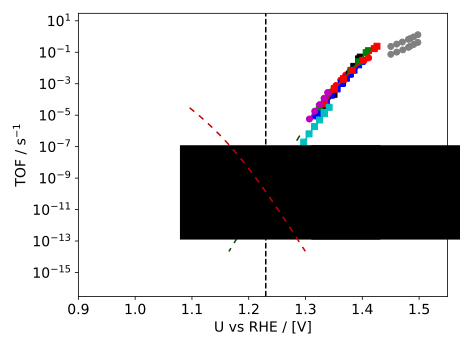
\includegraphics[width=0.6\textwidth]{04_Oxygen/fig/Ru_TOF_zoomout.png}
	\caption{Zoomed out TOF plot showing actual OER data from Ru and \ch{RuO2} (Figure \ref{fig:Ru_TOF}b), centered at the OER/ORR equilibrium potential at 1 bar \ch{O2}. A hypothetical ORR curve for a catalyst with ORR activity symmetrical to \ch{RuO2}'s OER activity is shown to illustrate that ORR is negligible at OER potentials.}
	\label{fig:Ru_TOF_zoomout}
\end{figure}

Many fundamental studies of OER electrocatalysts involve electrochemical measurements in oxygen-saturated electrolyte. Indeed, the use of an overpotential referenced to 1.23 V vs RHE implies oxygen-saturated electrolyte, since the equilibrium potential is only 1.23 V vs RHE when reactants and products excluding \ch{(H+ + e- )} are at unit activity, namely 1 bar \ch{O2}. 



This is analogous to hydrogen evolution reaction (HER) studies, in which a hydrogen-saturated electrolyte is used. For the case of HER, which is reversible on the best catalysts such as platinum, the use of hydrogen-saturated electrolyte makes a crucial difference. Indeed, a significant hydrogen evolution current can be measured at 0 V vs RHE if the hydrogen is transported away from the electrode surface (Subsection \ref{subsec:isotope_RHE}). The importance of having the hydrogen-saturated electrolyte is that HER and the reverse reaction, the HOR, both occur at appreciable rates at the equilibrium potential.

\begin{figure}[t!]
	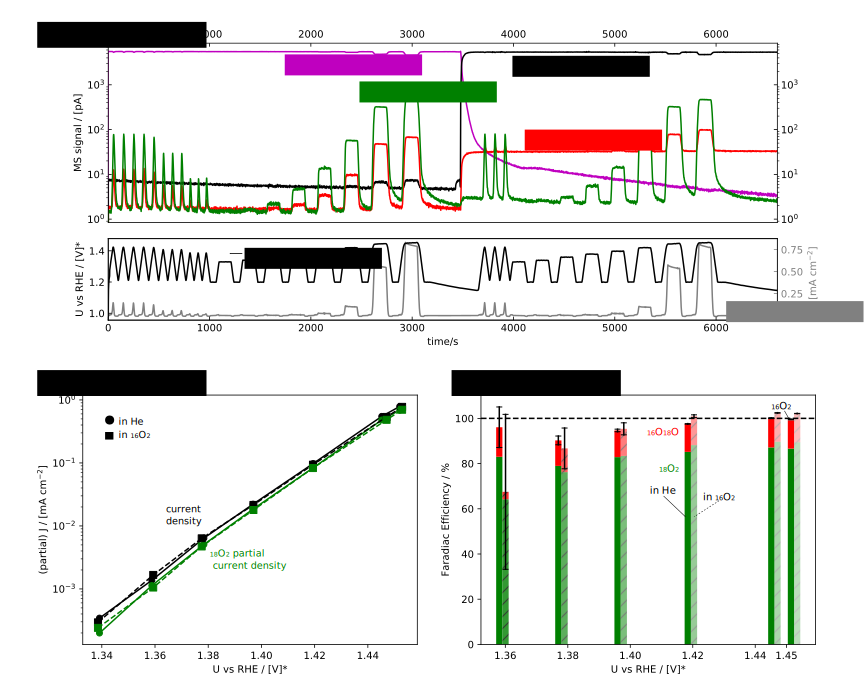
\includegraphics[width=1\textwidth]{04_Oxygen/fig/O2_vs_He_experiment_combined.png}
	\caption{\textbf{Activity of crystalline \ch{RuO2} in He-saturated and \ch{^{16}O2}-saturated 0.1 M \ch{HClO4} in \ch{H2^{18}O}.} \textbf{(a)} Experiment as an EC-MS plot. \textbf{(b)} The current density (black) and the partial current density for \ch{^{18}O} (green) at the end of each constant-potential step. \textbf{(c)} The Faridaic efficiencies for \ch{^{18}O2} (green) and \ch{^{16}O^{18}O} (red) as a function of potential. The error bar represents the uncertainty due to the standard deviation of the baseline m/z=34 MS signal.}
	\label{fig:He_vs_O2}
\end{figure}

However, at potentials sufficient to drive the highly irreversible OER, the equally irreversible oxygen reduction reaction (ORR) is negligible. This is abundantly clear when looking at Figure \ref{fig:Ru_TOF_zoomout}. Even if \ch{RuO2} was a symmetrical catalyst, i.e., as good at OER as ORR, the ORR current would still be approximately four orders of magnitude lower than the OER current at the  lowest potential at which we could detect \ch{O2} evolution, 1.29 V vs RHE. Furthermore, the scaling relations in oxygen evolution catalysts imply that a near-optimal OER catalyst like \ch{RuO2} is a rather bad ORR catalyst\cite{Busch2016}. 

Nonetheless, we decided to check if \ch{O2} saturation of the electrolyte had an effect. The use of isotope-labeled electrolyte enables the measurement by mass spectrometry of oxygen evolution under \ch{O2}-saturated conditions. Figure \ref{fig:He_vs_O2}a shows such an experiment. The activity of a crystalline \ch{RuO2} electrode is first measured in labeled electrolyte saturated with inert gas. At approximately 3500 s, the electrolyte is quickly saturated with natural \ch{O2} through the membrane chip, and the activity experiment is repeated. The m/z=36 (\ch{^{18}O2}) signal looks identical in the two activity measurements, whereas the background of the m/z=34 (\ch{^{16}O^{18}O}) is shifted up due to the natural isotopic distribution in the \ch{O2} carrier gas. 

The results are grouped by potential in Figure \ref{fig:He_vs_O2}b and c. There is no significant difference due to the presence of natural \ch{O2} in the current density or \ch{^{18}O2} partial current density (Figure \ref{fig:He_vs_O2}b). The increasing relative difference of the \ch{^{18}O2} partial current density and the total current density at smaller overpotential can be attributed to residual electrode charging current during the last 30 seconds of each constant potential step. \ch{O2} saturation of the electrolyte makes no significant difference in the Faradaic efficiency towards \ch{^{16}O^{18}O} (Figure \ref{fig:He_vs_O2}c), though the error bars in \ch{O2}-saturated electrolyte are much larger due to the m/z=34 background. Interestingly, the total labeled oxygen signal for the highest potentials, where the relative influence of background MS signal and electrode current loss to electrode charging are smallest, appears approximately 3\% larger in the \ch{O2}-saturated electrolyte. This is probably due to an artifact whereby the small flux of \ch{O2} carrier gas into the vacuum chamber influences the overall sensitivity of the mass spectrometer (see Subsection \ref{subsec:MS_theory}). That approximately 12\% of the combined \ch{O2} signal is \ch{^{16}O^{18}O} reflects the composition of the electrolyte which is approximately 6\% \ch{^{16}O} after addition of \ch{HClO4}.

The fact that the presence of \ch{O2} has no influence on the overall OER current density of the catalyst should be expected, as the ORR current density is insignificant at potentials at which OER is significant. However, the same cannot be said for the individual steps of the reaction, for which the reverse elementary reaction might occur at a non-negligible rate. Thus, lack of a significant effect on the isotopic makeup of the evolved oxygen does have a mechanistic implication, if an unsurprising one: the limiting step in OER does not come before the formation of the O-O bond. If the limiting step were prior to the formation of the O-O bond, then the O-O bond-forming step and all subsequent steps (Reactions \ref{rxn:OER_s3} and \ref{rxn:OER_s4}) would be at equilibrium. There would then be a non-negligible rate for adsorption and dissociation of \ch{^{16}O2}, and recombination of the adsorbed \ch{^{16}O} with \ch{^{18}O} from the electrolyte, giving an increased \ch{^{16}O^{18}O} signal in the evolved oxygen. This does not appear to be the case at $U\ge1.42$ V vs RHE, though below this potential the uncertainty due to the m/z=34 background is too great to draw any conclusions. 

In this Section, I described the use of isotope-labeled electrolyte to take advantage of the low background signal for \ch{^{18}O2} and thus lower the overpotential at which electrochemically produced oxygen can be detected and quantified. In this final Subsection, I used the lack of scrambling in \ch{^{16}O2}-saturated \ch{H2^{18}O} electrolyte to probe the rate-determining step of the OER an \ch{RuO2}. Both of these uses of isotope labeling in OER research are novel to the best of my knowledge. However, isotope labeling has been used extensively to probe another phenomenon: the involvement of lattice oxygen in the oxygen evolution reaction. This is the subject of the next Section.